\documentclass[11pt]{scrartcl}

\usepackage[top=1in, bottom=2cm, left=1in, right=1in]{geometry}
\usepackage{graphicx}
\usepackage{amsmath}

\begin{document}

\title{Project 1 STAT5376}
\subtitle{Bayesian Analysis of Noisy Images}
\author{Li Sun}
\date{\today}
\maketitle

\noindent
1. Goal: Given observed noisy images, our goal is to perform a Bayesian analysis of this data. We will assume a prior probability model and an observation model to obtain a posterior density, and will generate samples from the posterior.

\bigskip

\noindent
2. Models\\
(a)Prior Model: \\
$$f(I_{i,j}|\text{all other pixels})=f(I_{i,j}|I_{i,j-1},I_{i-1,j},I_{i+1,j},I_{i,j+1})=N(m,\sigma^2_1)$$
All conditional density of a pixel of this m by n Markov Random field only depends on 4 adjacent pixels, 3 for edge pixels and 2 for corner pixels. The m is mean of all neighbors\\

\begin{center}
$
\Pi =
\begin{bmatrix}
0.2&0.2&0.1&0.5\\
0.1&0.3&0.4&0.2\\
0.3&0.2&0.3&0.2\\
0.1&0.3&0.1&0.5\\
\end{bmatrix}
$
\end{center} 
Generates 4 sample path of MC, put relative frequency with which the path visits the four states for i up to 1000.\\
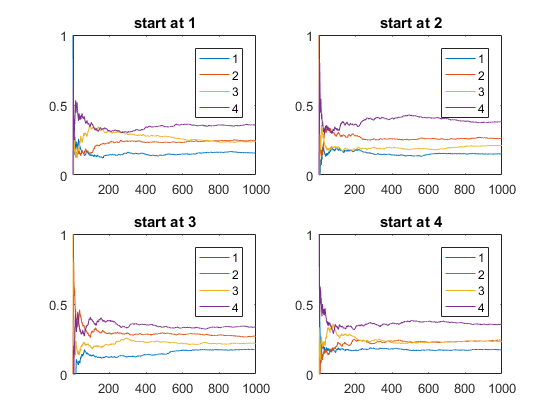
\includegraphics[scale=1]{hw2p1.png}
The re-scaled dominant eigenvector is [0.1607 0.2616 0.2231 0.3546]\\
The simulated frequence starts from '1' is [0.157 0.246 0.24 0.357](if starts from other states, results are similar)\\ 
They are very close.\\


\bigskip

2. Do similar thing for another 2 $\Pi$\\
For the first $\Pi$ which is reducible. we got\\
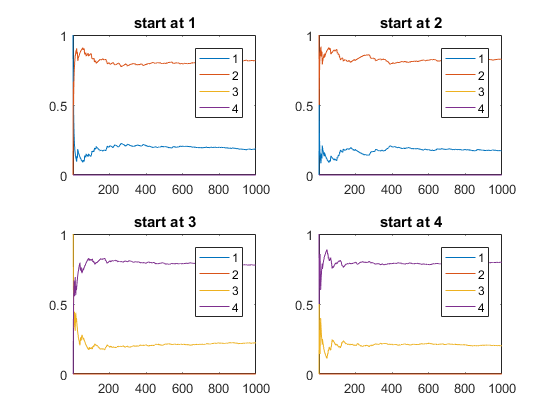
\includegraphics[scale=1]{hw2p2.png}
1.This $\Pi$ is reducible because states 1, 2 are not communicating with states 3 and 4. So with different starting value we will get different stationary pmf.Theoretically we can divide this $\Pi$ into 2 small $\pi$ with dimension 2 by 2. We can calculate the theoretical stationary pmf of this two MC. If we start with 1 or 2. pmf1 is (0.1667, 0.8333, 0, 0), if we start with 3 or 4, the pmf2 is (0,0, 0.2222, 0.7778). As shown in the 1000 step convergence, which is very close to theoretical ones calculated from the eigenvectors\\

\bigskip

For the second $\Pi$ whose periodicity is 2. we got\\
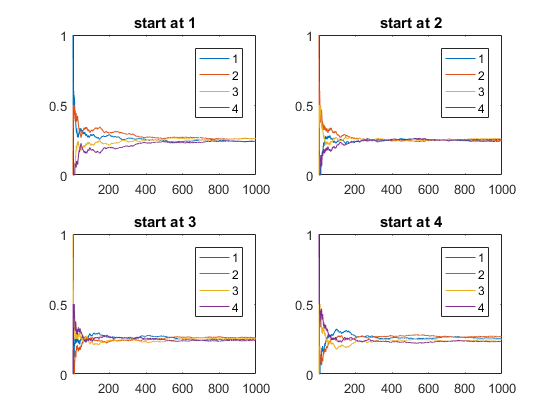
\includegraphics[scale=1]{hw2p3.png}

The second $\Pi$ is periodic with period 2 for all states. So at each step, the pmf is always different if the current stats is different. This is like a process of moving a block in a 2 by 2 grid, the 4 possible location of the block is coded as 1,2,3,4 and the block has to move and only can move 1 step to one of its two neighbor locations. The probability of moving this block to either one is always equal. After a number of steps, we can find the probability for each location the block stays are equal. The simulated stationary pmf is roughly 0.25 for each states and the the pmf calculated from eigenvector is (0.25 0.25 0.25 0.25), they match.\\

\bigskip

3. Let $X_t$ be a MC generated using some initial probability P[1] and the transition matrix $\Pi$ is:\\
\begin{center}
$
\Pi=
\begin{bmatrix}
0.1&0.3&0.4&0.2\\
0.2&0.1&0.3&0.4\\
0.4&0.2&0.1&0.3\\
0.3&0.4&0.2&0.1\\
\end{bmatrix}
$
\end{center}
i)the above matrix is irreducible because all elements are communicating with each other\\
ii)the above matrix is aperiodic because $period(a_1)=1$ and all states share the same period because of i), so it is aperiodic.\
The stationary probability is found by re-scale the right eigenvector with eigenvalue is 1. It is (0.25,0.25,0.25,0.25).\\
For the second part, the right side can be calculated as
$$\sum_{j=1}^4f(a_j)P(a_j)=E(f(aj))=1.125$$
So this is to prove the mean of $f(X_i)$ where $X_i$ is MC with stationary pmf P, is asymptotically equal to the $E(f(a_i))$ were $a_i$ are from pmf P.\\
Simulation:\\
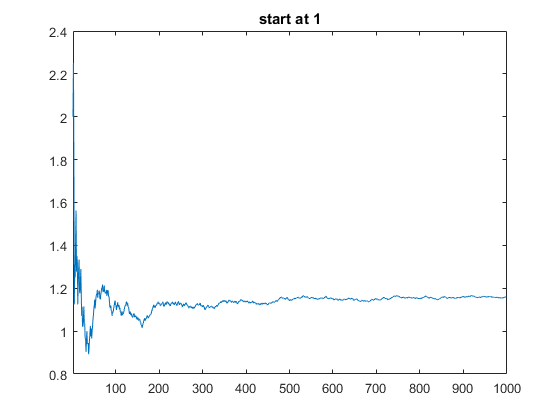
\includegraphics[scale=1]{hw2p4.png}\\
This shows that expected value is converging to 1.125 as expected.\\

\bigskip

All code please see https://github.com/rikku1983/STAT5376\\
\bigskip

Thanks!


\end{document}